\section{问题设定}

\subsection{多帧观测模型}

考虑一台 \eng{LWIR} 长波红外相机对芯片进行微扫描成像。电动台以亚像素步长在二维光栅网格上逐帧平移场景，
共采集 \(K\) 帧低分辨率（\eng{LR}）温度矩阵。设 \(x \in \mathbb{R}^N\) 为待恢复的高分辨率（\eng{HR}）温度图像
（定义在 \(2\times\) 输出网格上），第 \(k\) 帧观测建模为
\begin{equation}
  y_k = D\,B\,H\,S_{t_k}\,x + n_k,\quad k = 1,\ldots,K.
\end{equation}
各算子的级联关系如图~\ref{fig:obs-model}~所示。其中 \(S_{t_k}\) 按精修后的亚像素位移 \(t_k\) 对 \eng{HR} 网格作平移重采样；
\(H\) 为光学系统点扩散函数（\eng{PSF}）卷积，建模为高斯模型，标准差 \(\sigma\) 以
\eng{LR} 像素为单位（附录~A.5.2）；\(B\) 为探测器孔径的矩形积分；
\(D\) 为 \eng{HR}\(\rightarrow\)\eng{LR} 的降采样。\(n_k\) 表示探测器读出噪声，
标称尺度由 0.0724\,\(^\circ\)C 噪声底给出；热漂移、对齐残差与 \eng{PSF} 失配作为模型误差，
由会话门控与消融实验另行处理（附录~B）。
本文理论分析将 \(t_k\) 视为固定量；实际系统中它来自台位先验与数据驱动精修，
而不是将台位指令当作对齐真值。

将 \(K\) 帧联立，定义堆叠观测算子
\begin{equation}
  A =
  \begin{bmatrix}
    A_1 \\ \vdots \\ A_K
  \end{bmatrix},
  \qquad
  A_k = D\,B\,H\,S_{t_k}.
\end{equation}

\begin{figure}[t]
  \centering
  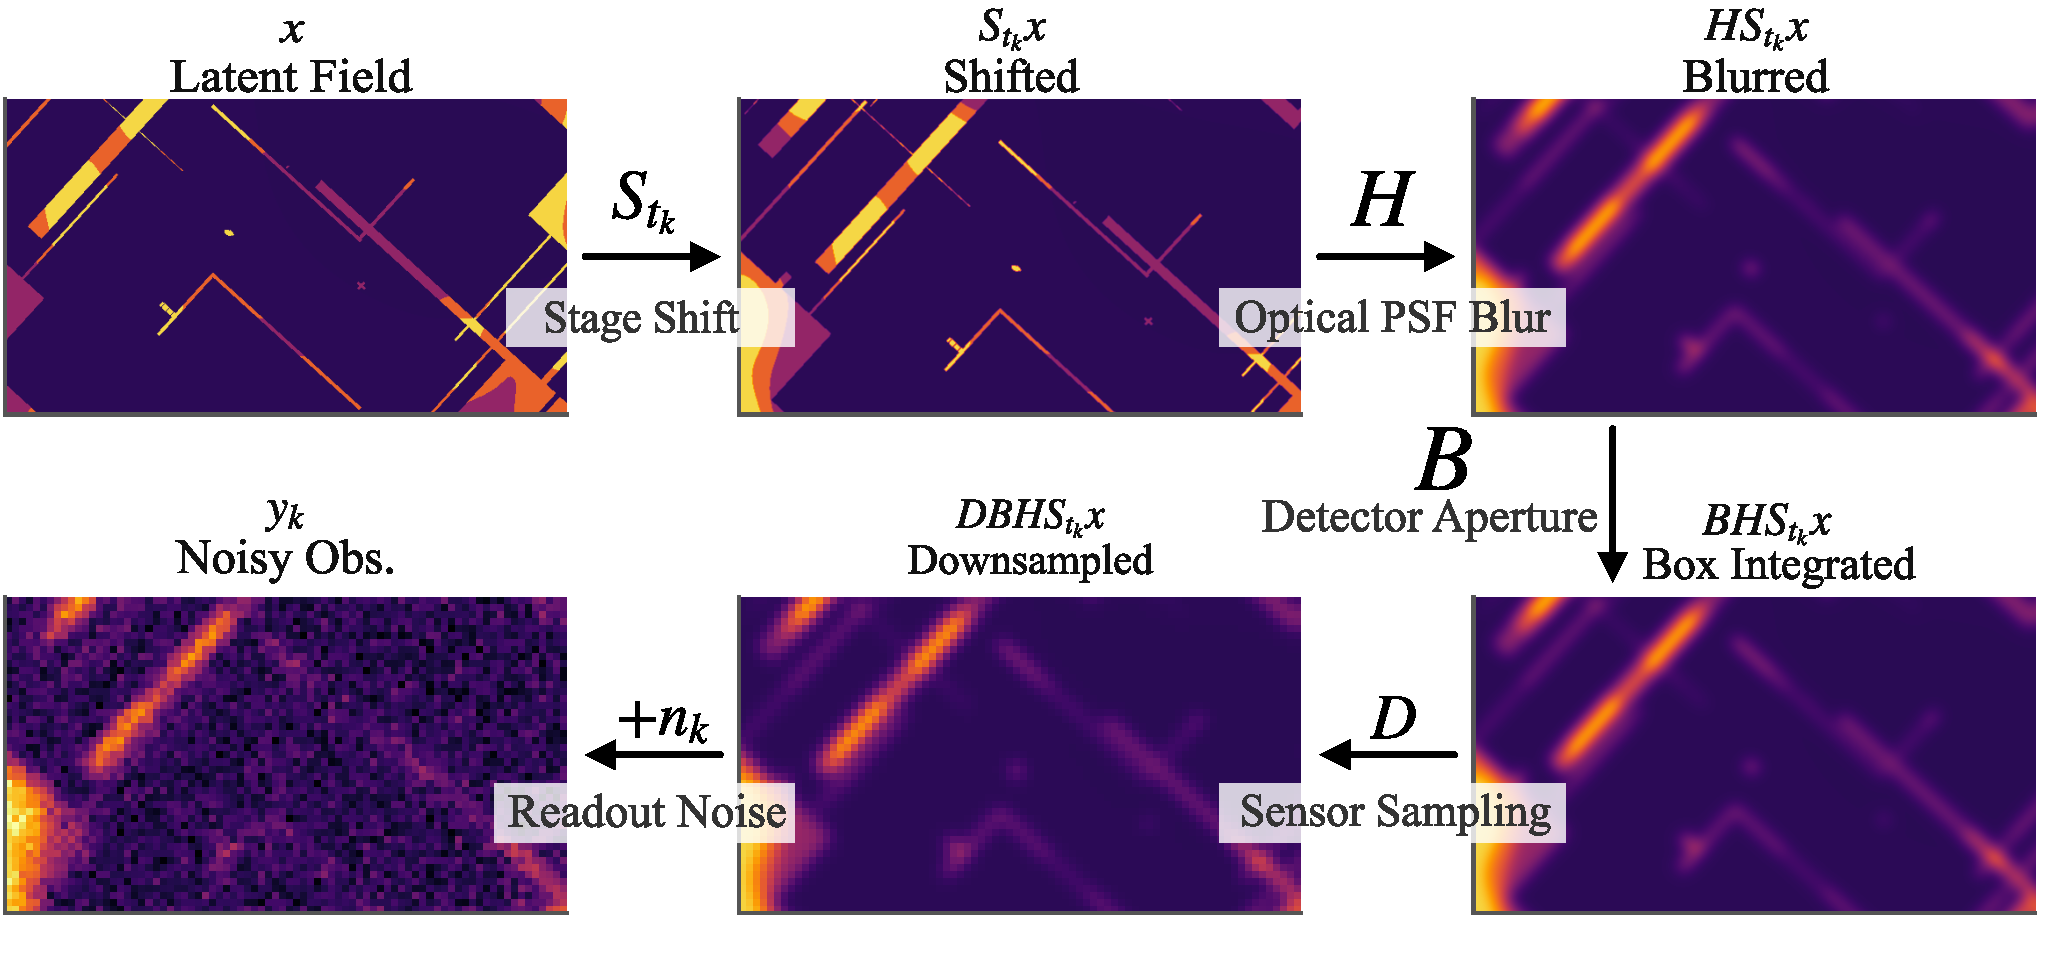
\includegraphics[width=\linewidth]{../figures/observation_pipeline.pdf}
  \caption{标定化观测模型示意：单帧算子链 \(S_{t_k}\!\to\!H\!\to\!B\!\to\!D\) 与 \(K\) 帧堆叠算子 \(A\)。}
  \label{fig:obs-model}
\end{figure}

\(A\) 的结构——带限衰减特性、降采样引起的混叠折叠、以及二者共同产生的零空间——决定了
哪些 \eng{HR} 信息可被观测约束，哪些超出观测能力。下一节对此展开分析。


\begin{figure*}[t]
  \centering
  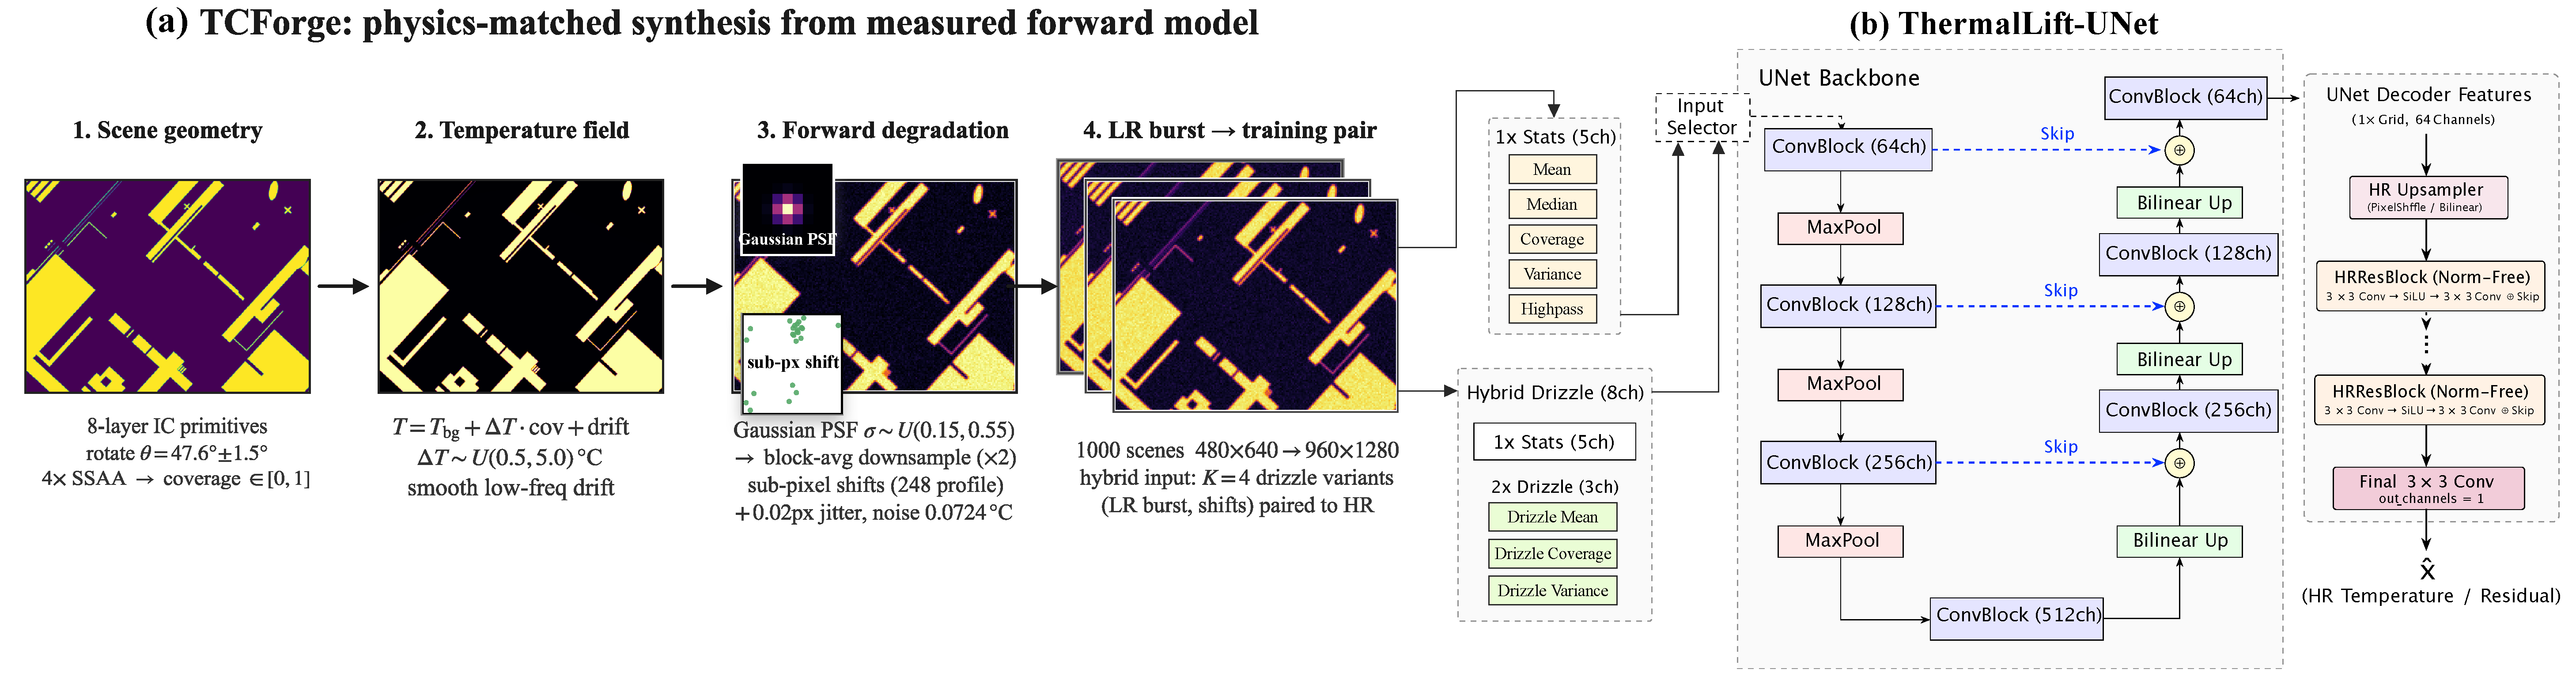
\includegraphics[width=\textwidth]{../figures/fig_tcforge_pipeline.pdf}
  \caption{(a) \eng{TCForge} 物理匹配合成管线：以标定前向模型为核心，
    经 场景几何$\to$温度场渲染$\to$前向退化$\to$训练对 四阶段生成合成训练数据；
    (b) \eng{ThermalLift-UNet} 网络结构：左侧为输入选择器（\(1\times\) 统计 5 通道
    或 \eng{hybrid drizzle} 8 通道），中部为共享 \eng{UNet} 骨干，
    右侧为无归一化高分残差细化模块与最终 \eng{HR} 温度/残差输出。}
  \label{fig:method-pipeline}
\end{figure*}

\subsection{可恢复性边界}

在讨论 \eng{HR} 信息的可恢复性之前，需要区分三个相关但含义不同的空间尺度：
物方采样间距（探测器在样品平面上的每像素长度，本系统为 10\,\(\mu\)m）；
空间分辨率（由光学衍射、\eng{PSF} 与探测器孔径共同决定的最小可分辨结构尺度）；
输出网格采样（\(2\times\) 重建网格的像素间距，即 5\,\(\mu\)m）。
三者是不同的物理量——更密的输出网格提供了更精细的采样格点，但不改变光学系统所决定的空间分辨率。

堆叠算子 \(A\) 中的不可观测方向来自两个机制。
其一为带限衰减：光学 \eng{PSF} 与探测器孔径构成的预采样传递函数在高频段强烈衰减，
将超过截止频率的分量压到噪声以下。
其二为混叠折叠：降采样 \(D\) 将多个 \eng{HR} 频率映射到同一 \eng{LR} 频带，
部分高频组合在折叠后相消。
多帧相位多样性通过增加约束方程可缩小精确零空间并改善覆盖良好的混叠块的条件数，
但无法恢复被所有帧共同的预采样传递函数消灭的频率分量（严格推导见附录~A.2）。

具体地，\(A\) 的零空间
\begin{equation}
  \ker(A) = \bigcap_{k=1}^K \ker(A_k)
\end{equation}
包含所有使 \(K\) 帧观测完全不变的 \eng{HR} 扰动。精确零空间之外，\(\epsilon\)-零空间
\begin{equation}
  \mathcal{N}_\epsilon = \mathrm{span}\{v_i:\sigma_i \le \epsilon\}
\end{equation}
（\(\sigma_i\) 为 \(A\) 的奇异值）刻画近似不可见的方向：在这些方向上，观测域损失的灵敏度随
\(\sigma_i \to 0\) 消失；对平方损失而言，恢复曲率随 \(\sigma_i^2\) 消失（附录~A.2 命题~P2--P3）。

这一性质直接限制了前向一致性作为质量指标的辨别能力。任何通过固定算子 \(A\) 比较预测与观测的损失函数，
对 \(\ker(A)\) 中分量完全不变，对 \(\mathcal{N}_\epsilon\) 中分量仅有 \(O(\epsilon)\) 量级的弱响应。
施加有界频带加权（\eng{highpass}、全频带或其他形式）只能将上界放大有限常数因子，
无法在近零奇异值方向制造非消失的恢复力。
因此，低前向残差只能作为观测域完整性检验，不能单独证明 \eng{HR} 细节忠实，
也不能在无真值条件下排序检查点。

系统的可传递频带由 \eng{MTF}--\eng{SNR} 共同约束（附录~A.1）；这一判据是 \eng{SR} 可行性的必要条件，
但不是充分条件——它只保证信息在传递链中未被完全消灭，却不保证在模型失配与热漂移下仍可可靠恢复。
上述分析对 \(2\times\) 网格上的重建结果施加了三项不可绕过的解读约束：
\begin{enumerate}
  \item 输出网格的 5\,\(\mu\)m 采样间距不等于 5\,\(\mu\)m 空间分辨率——后者由光学系统决定，更密的网格仅提供更精细的采样格点；
  \item 在 \eng{HR} 真值缺失的条件下，温度计量级精度无法由观测域损失验证；
  \item 位于分辨率极限附近的最细结构落入 \(\mathcal{N}_\epsilon\)，其恢复不具备充分的观测域支撑。
\end{enumerate}
因此，后文的实验评估以轮廓可见性与重建稳定性为判据，而非分辨率或精度的绝对声明。

\subsection{评估指标简介}

后文采用三类无真值指标。

\paragraph{分半 \eng{FRC}.}
将 248 帧按亚像素相位分层拆成子集 \(A\)、\(B\)，各自独立重建后计算频域环状相关：
\begin{equation}
  \mathrm{FRC}(r) = \frac{\displaystyle\sum_{|\mathbf{f}| \in r} \mathrm{Re}\bigl(F_A(\mathbf{f}) \cdot \overline{F_B(\mathbf{f})}\bigr)}
  {\sqrt{\displaystyle\sum_{|\mathbf{f}| \in r} |F_A(\mathbf{f})|^2 \;\cdot\; \sum_{|\mathbf{f}| \in r} |F_B(\mathbf{f})|^2}}
\end{equation}
其中 \(F_A\)、\(F_B\) 为两半重建的二维傅里叶变换，\(r\) 为频率环半径。
\eng{FRC} 衡量两半在各频带的一致性；分层设计与控制组见附录~A.4。

\paragraph{代理指标对.}
将重建输出变换到高通域 \(u = \hat{x} - G_{\sigma_{\mathrm{bg}}}(\hat{x})\)（\(\sigma_{\mathrm{bg}} = 5\) \eng{HR} px），
控制图 \(c\) 为 248 帧均值的 bicubic 上采样经同一变换。在此基础上定义伪影分数 \(\artscore(u)\) 与原始控制相关性 \(\mathrm{corr}(u)=\mathrm{Pearson}(u,c)\)，其中
\begin{equation}
  \artscore(u) = \frac{\mathrm{std}\bigl(h(u)\bigr) + 0.25 \cdot \mathrm{std}(\nabla^2 u)}{\mathrm{std}(u)},\quad h(u)=u-G_{\sigma\!=\!1}(u).
\end{equation}
\(\artscore(u)\) 度量 \(u\) 内部更高频能量的占比，\(\mathrm{corr}(u)\) 衡量重建高通结构与保守观测锚的一致程度。
二者构成漂移温度计与选点准则（构造性反相关论证见附录~A.3）。

\paragraph{锯齿走线剖面.}
在固定中心锯齿走线横截面上测量半高全宽（\eng{FWHM}）与凹陷深度（\eng{dip depth}），
用于结构级轮廓门控（完整协议见附录~C.6）。

